\chapter{Evaluation}
This chapter details how the knowledge graph is evaluated upon completion. 

\section{Knowledge Graph Quality Assessment}
\hspace{0.5cm} Assessment knowledge graph quality is important to ensure the produced knowledge graph is valid and correct, using \cite{knowledgegraphevaulationbook} as guidance to assess knowledge graph quality.

The main four sections used to assess knowledge graph quality are: 

\begin{itemize}
    \itemsep0em 
    \item Accuracy
    \item Coverage
    \item Coherency
    \item Succinctness
\end{itemize}

For each section, generated knowledge graphs for five different organs will be used to measure overall quality. Organs to be tested from the dataset are: \textit{Part14\_000Brouwershaven}, \textit{Part14\_000Niezijl}, \textit{Part14\_000Folsgare}, \textit{Part14\_000GravenhageNoorderkerk} and \textit{Part14\_000Groede}. For simplicity, a random sample of five was selected from the list of organ codes and the produced knowledge graphs will represent the quality of all possible organs. Generating the knowledge graphs and assessing the quality from the output files was the method employed. 

\subsection{Accuracy}
\hspace{0.5cm} "Accuracy refers to the extent to which entities and relations- encoded by nodes and edges in the graph- correctly represent real-life phenomena". \cite{knowledgegraphevaulationbook}. In this context, accuracy means that the knowledge graph generated (both subjects and relationships) needs to correctly reflect the relationships between the organ topic. 

There are three types of accuracy: 
\begin{itemize}
    \itemsep0em 
\item Syntactic Accuracy.
\item Semantic Accuracy.
\item Timeliness.
\end{itemize}

\subsubsection{Syntactic Accuracy}
\hspace{0.5cm} Syntactic accuracy refers to whether the data presented is valid for it's given type. \cite{knowledgegraphevaulationbook}

\noindent An example of a potential violation: 
\begin{lstlisting}
    "This is an organ" would be incompatible with xsd:integer.
\end{lstlisting}

Upon assessing the produced knowledge graphs for each of the five organs, no syntactic inaccuracies were found. Due to the ontology being derived off the provided ontology and the external links, all resulting knowledge graphs did not contain any syntactic inaccuracies. 

\subsubsection{Semantic Accuracy}
\hspace{0.5cm} Semantic accuracy refers to whether data values are being correctly represented in the context of the real world. \cite{knowledgegraphevaulationbook}

\noindent An example of a potential violation: 
\begin{lstlisting}
    Date of build (for an organ) coming after today's date. 
\end{lstlisting}

In regards to semantic accuracy, none of the five organs contained inaccuracies in this context. This can be explained for the same reasons as the lack of syntactic inaccuracies. 

\subsubsection{Timeliness}
\hspace{0.5cm} Timeliness refers to how up-to-date or relevant the knowledge graph is with the real current state of the modern world. \cite{knowledgegraphevaulationbook}

\noindent An example of a potential violation: 
\begin{lstlisting}
    Organ's location stated as "Netherlands", but has been moved recently to Portugal and the knowledge graph has not been updated.
\end{lstlisting}

In the produced knowledge graphs, violations of timeliness can occur due to the static nature of the dataset. An example of a violation may occur when the ?organDivisionName is no longer the organ's current disposition in real life, but the data in the dataset does not update. This particular violation, will occur over time as the organ changes over time. At the time being, no timeliness violations occur in the produced knowledge graphs.

\subsection{Coverage}
\hspace{0.5cm} "Coverage refers to avoiding the omission of domain-relevant elements, which may yield incomplete results". \cite{knowledgegraphevaulationbook}

In this context, the knowledge graph result must have completely fill the ontology framework required in all of it's nodes and edges. This is to accurately represent the entire dataset given. 

There are two types of coverage: 
\begin{itemize}
\itemsep0em 
\item Completeness.
\item Representativeness.
\end{itemize}

\subsubsection{Completeness}
\hspace{0.5cm} Completeness ensures the knowledge graph is correctly filled with all the relevant information present in a particular dataset. \cite{knowledgegraphevaulationbook}

Some examples of violations: 
\begin{lstlisting}
    - A organ classes lacking information

    - Important values being missing for a specific organ property. 
\end{lstlisting}

\subsubsection{Representativeness}
\hspace{0.5cm} Representativeness ensures the knowledge graph does not involve any bias and it does not exclude anything relevant. \cite{knowledgegraphevaulationbook}

Some examples of violations: 
\begin{lstlisting}
    - Under-represent organs from other parts of the world.
    
    - Under-represent organ data from other languages.

    - Under-represent people (organist, owner etc.) from a particular gender or race etc.
\end{lstlisting}

\subsection{Coherency}
\hspace{0.5cm} "Coherency refers to how well the knowledge graph conforms to the formal semantics and constraints defined at schema level". \cite{knowledgegraphevaulationbook}

In this context, the knowledge graph result must follow the dataset and accurately display the data appropriately. 

There are two types of coherency:
\begin{itemize}
    \itemsep0em 
\item Consistency
\item Validity
\end{itemize}

\subsubsection{Consistency}
\hspace{0.5cm} Consistency ensures the knowledge graph does not involve any contradictions with regard to logic. \cite{knowledgegraphevaulationbook}

An example of a violation: 
\begin{center}
    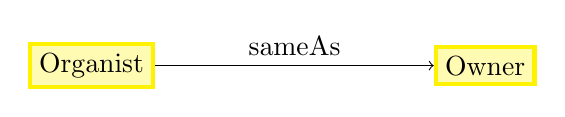
\begin{tikzpicture} [
        square/.style={draw=yellow, rectangle, ultra thick, fill=yellow!30},
        align=center,
        node distance=5cm ]
    \node[square] (q1)  {Organist};
    \node[square, right of=q1] (q2)  {Owner};
    \draw (q1) edge[->,above] node {sameAs} (q2);
    \end{tikzpicture}
\end{center}

\begin{center}
    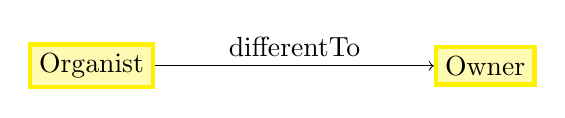
\begin{tikzpicture} [
        square/.style={draw=yellow, rectangle, ultra thick, fill=yellow!30},
        align=center,
        node distance=5cm ]
    \node[square] (q1)  {Organist};
    \node[square, right of=q1] (q2)  {Owner};
    \draw (q1) edge[->,above] node {differentTo} (q2);
    \end{tikzpicture}
\end{center}

This is an example of a contradiction because, logically, an organist can not be both: the same as and different to the owner. Note that data is not input into the classes for explanation purposes.

\subsubsection{Validity}
\hspace{0.5cm} Validity means that the resulting knowledge graph does not include any constraint violations, with respect to the shapes involved. \cite{knowledgegraphevaulationbook}

An example of a violation:
\begin{center}
    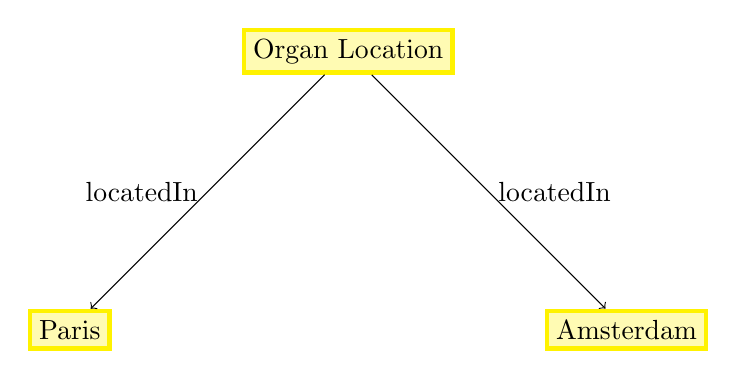
\begin{tikzpicture} [
        square/.style={draw=yellow, rectangle, ultra thick, fill=yellow!30},
        align=center,
        node distance=5cm ]
    \node[square] (q1)  {Organ Location};
    \node[square, below right of=q1] (q2)  {Amsterdam};
    \node[square, below left of=q1] (q3)  {Paris};

    \draw (q1) edge[->,right] node {locatedIn} (q2);
    \draw (q1) edge[->,left] node {locatedIn} (q3);
    \end{tikzpicture}
\end{center}

This example is a violation because "Organ Location"'s constraints have only one node as an Organ can only be in one location at once. Therefore, there can only be one city branching out of the node 'Organ Location'.

\subsection{Succinctness}
\hspace{0.5cm} "Succinctness refers to the inclusion of relevant content that is represented in a concise and intelligible manner." \cite{knowledgegraphevaulationbook}

In this context, it means the knowledge graph created should be easily understandable and to the point. 

There are three types of succinctness: 
\begin{itemize}
    \itemsep0em 
\item Conciseness.
\item Representational Conciseness.
\item Understandability.
\end{itemize}

\subsubsection{Conciseness}
\hspace{0.5cm} Conciseness refers to the need of avoiding the input and addition of irrelevant data into the dataset, and subsequently, into the knowledge graph. \cite{knowledgegraphevaulationbook}

An example of a violation: 
\begin{lstlisting}
    Adding information about musicians that is not relevant to organs.
\end{lstlisting}

\subsubsection{Representational Conciseness}
\hspace{0.5cm} Representational conciseness refers to the extent to which the knowledge graph content is compactly represented. \cite{knowledgegraphevaulationbook}

An example of a violation: 
\begin{lstlisting}
    Containing two properties that serve the same purpose i.e.:
        - Organist
        - Organ Player
\end{lstlisting}
\begin{center}
    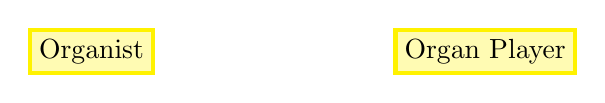
\begin{tikzpicture} [
        square/.style={draw=yellow, rectangle, ultra thick, fill=yellow!30},
        align=center,
        node distance=5cm ]
    \node[square] (q1)  {Organist};
    \node[square, right of=q1] (q2)  {Organ Player};
    \end{tikzpicture}
\end{center}

Note that the actual names of the organist and organ player are not in the example nodes of the knowledge graph for explanation purposes. 

\subsubsection{Understandability}
\hspace{0.5cm} Understandability refers to the need for readability and ease of understanding the knowledge graph generated. \cite{knowledgegraphevaulationbook}

An example of a violation: 
\begin{lstlisting}
    Using property names such as Organist 1, when asked to state the name of an organist. (We should use their actual name instead)
\end{lstlisting}
\begin{center}
    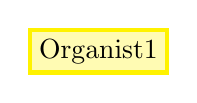
\begin{tikzpicture} [
        square/.style={draw=yellow, rectangle, ultra thick, fill=yellow!30},
        align=center,
        node distance=5cm ]
    \node[square] (q1)  {Organist1};
    \end{tikzpicture}
\end{center}
